%
% $RCSfile: open_and_closed_loop.tex,v $
%
% Copyright (C) 2002-2008. Christian Heller.
%
% Permission is granted to copy, distribute and/or modify this document
% under the terms of the GNU Free Documentation License, Version 1.1 or
% any later version published by the Free Software Foundation; with no
% Invariant Sections, with no Front-Cover Texts and with no Back-Cover
% Texts. A copy of the license is included in the section entitled
% "GNU Free Documentation License".
%
% http://www.cybop.net
% - Cybernetics Oriented Programming -
%
% http://www.resmedicinae.org
% - Information in Medicine -
%
% Version: $Revision: 1.1 $ $Date: 2008-08-19 20:41:08 $ $Author: christian $
% Authors: Christian Heller <christian.heller@tuxtax.de>
%

\subsubsection{Open- and Closed Loop}
\label{open_and_closed_loop_heading}
\index{Open Loop Control System}
\index{Closed Loop Control System}
\index{Automation Engineering}
\index{Control Engineering}
\index{Feedback Control System}
\index{Controller}
\index{Linear Behaviour}
\index{Proportional Behaviour}
\index{Differential Behaviour}
\index{Integral Behaviour}

The scientific discipline of \emph{Automation-} and \emph{Control Engineering}
knows two kinds of control systems: \emph{Open Loop} and \emph{Closed Loop}
(\emph{Feedback}). German language better confines both by defining the terms
\emph{Steuerung} (stearing) and \emph{Regelung} (controlling). Figure
\ref{blackbox_figure} illustrates a closed loop system, received by adding a
feedback loop to the black box mentioned before.

\begin{figure}[ht]
    \begin{center}
        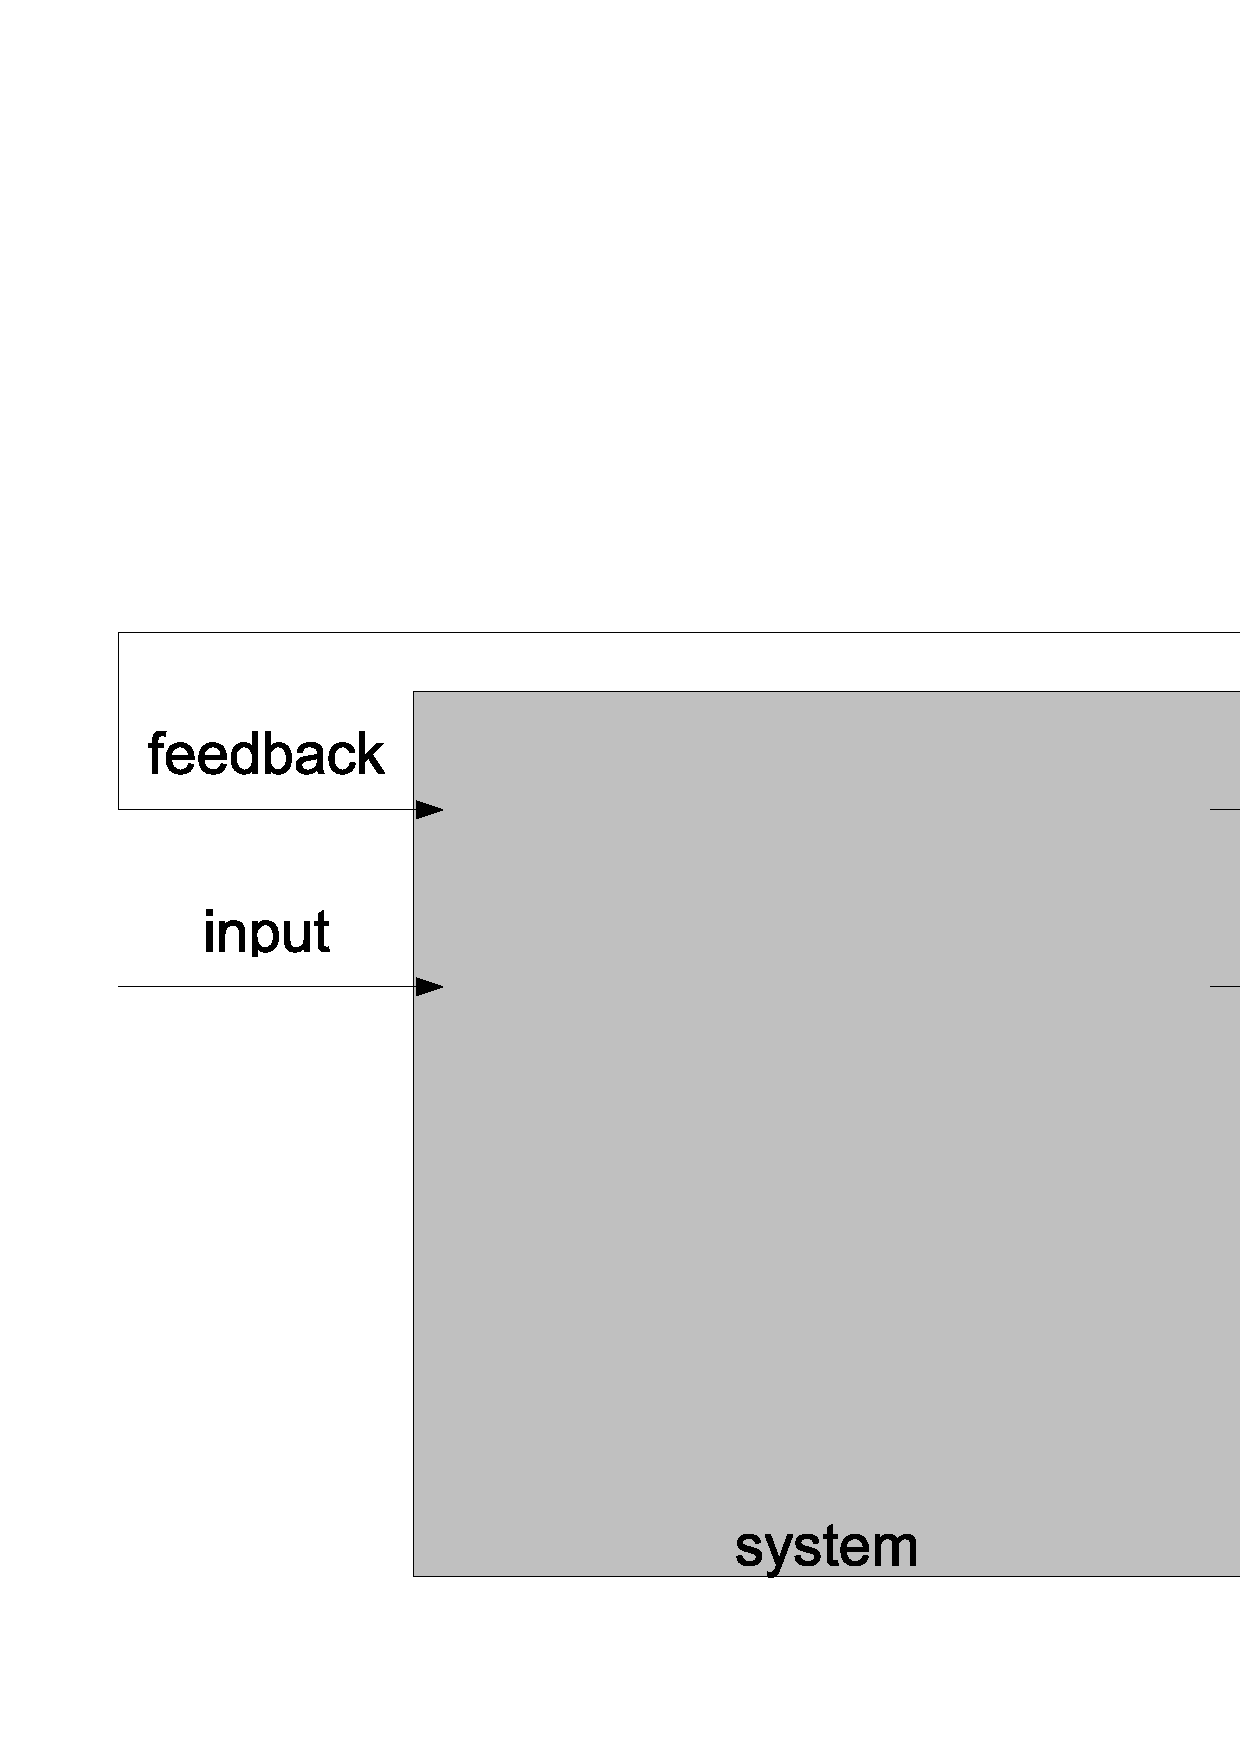
\includegraphics[scale=0.3,angle=-90]{graphic/blackbox.pdf}
        \caption{Closed Loop System with Feedback, modelled as Black Box}
        \label{blackbox_figure}
    \end{center}
\end{figure}

\newpage

A device controlling the behaviour of a system is called a \emph{Controller}.
Automation engineering uses electronic components such as \emph{Capacitor} and
\emph{Coil} to build controllers providing \emph{linear} (proportional),
\emph{differential} or \emph{integral} behaviour. In software engineering,
things are simpler. A computer program containing special mathematical
equations can simulate and control a system.

A software system's internal signal processing loop reads signals one by one,
from a signal memory (section \ref{knowledge_management_system_heading}).
While processing them, new signals may get created and placed in the signal
memory. This is how output results may be fed back to become a new input to the
software system.
